\section{Aplicação Web}

\subsection{Software Utilizado}

A base de dados usada foi MongoDb.
A ligação a esta foi feita com a linguagem Python, a partir de uma ferramenta chamada PyMongo.
Para fazer a ligação ao front-end usamos uma framework chamada Flask.
Este por sua vez usou HTML, CSS, JavaScript e Jinja2.

\subsection{Funcionamento}

Ao abrirmos a nossa aplicação web é nos apresentado o seguinte ecrã, com filmes a passar.

\begin{figure}[H]
\centering
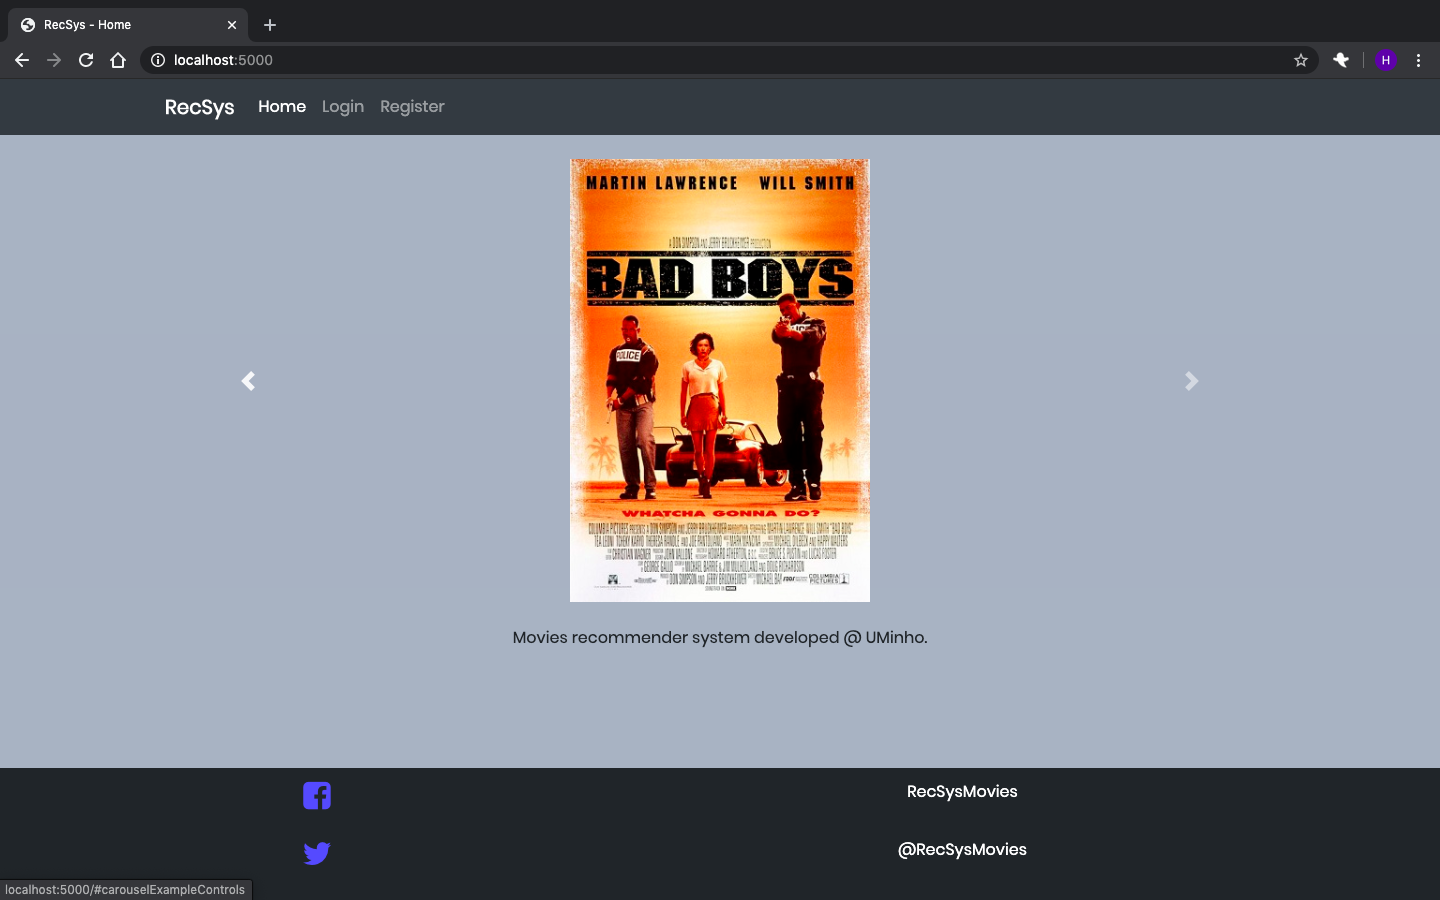
\includegraphics[scale=0.3]{1.png}
\end{figure}


Para o funcionamento desta aplicação é necessário fazer o Registo e de seguida Login.
\begin{figure}[H]
\centering
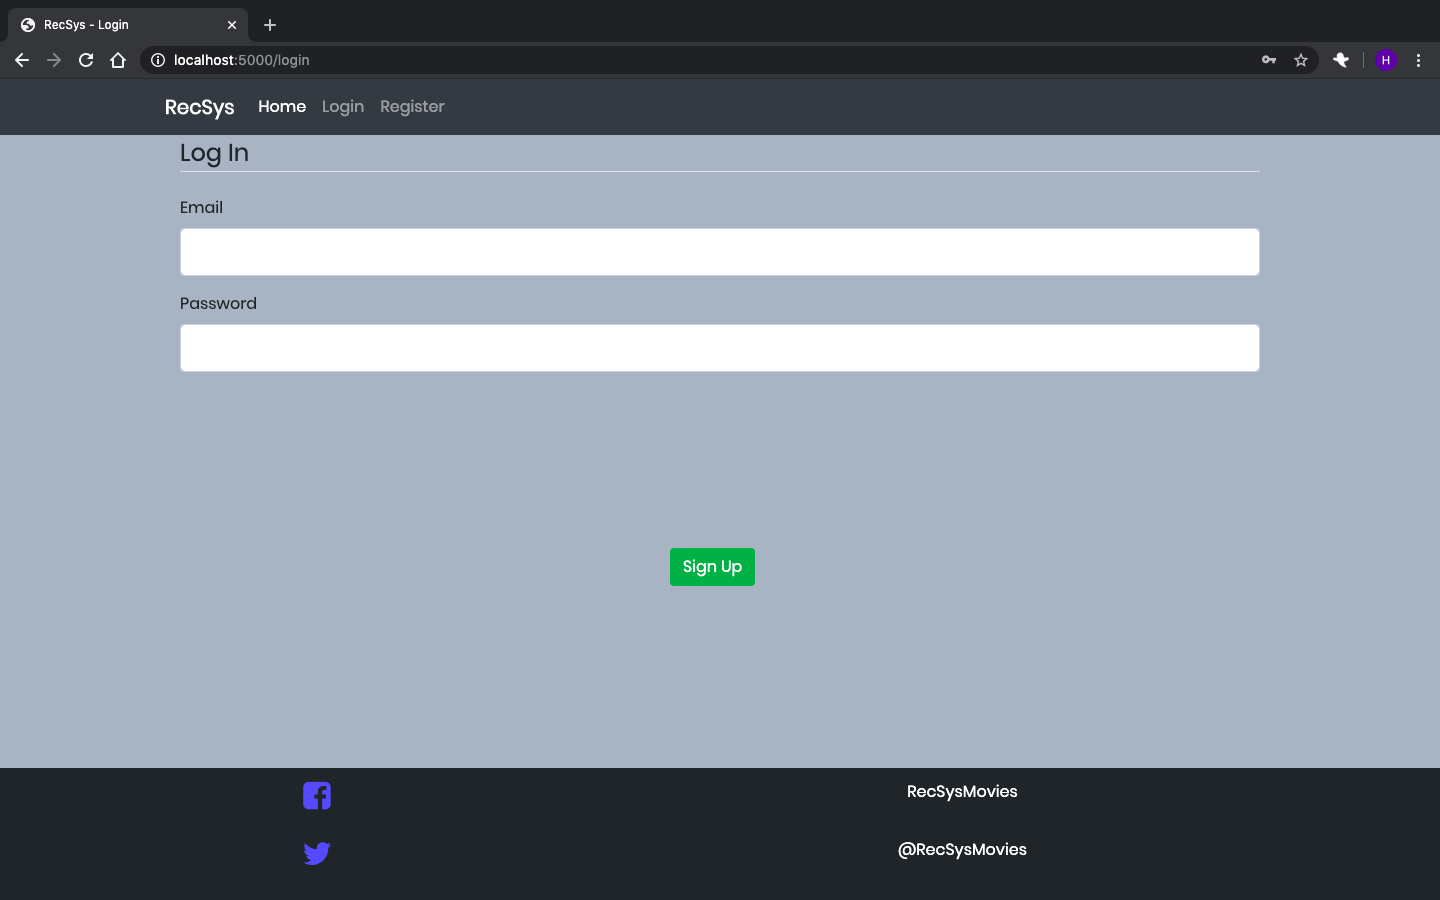
\includegraphics[scale=0.3]{2.png}
\end{figure}


Foi criada uma colecção em MongoDb designada de users que contem o nome de utilizador, e-mail e password fornecidos aquando do registo. Quando este é feito, é atribuído também um id.

Quando um utilizador faz login na sua conta pode ver os filmes existentes, bem como a sua pontuação e um breve resumo deste. É possível procurar filmes pelo ano de realização, género e tipo de recomendação. 

 \begin{figure}[H]
\centering
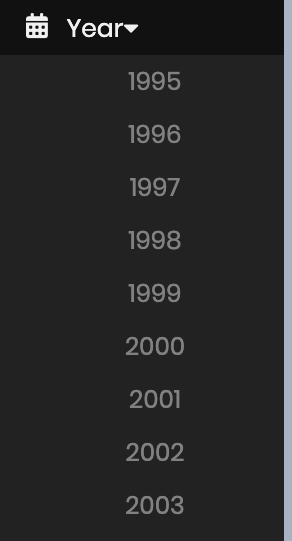
\includegraphics[scale=0.25]{7.png}
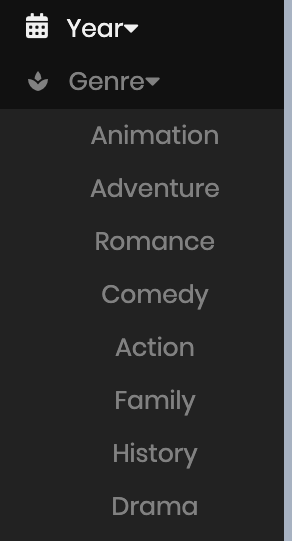
\includegraphics[scale=0.25]{8.png}
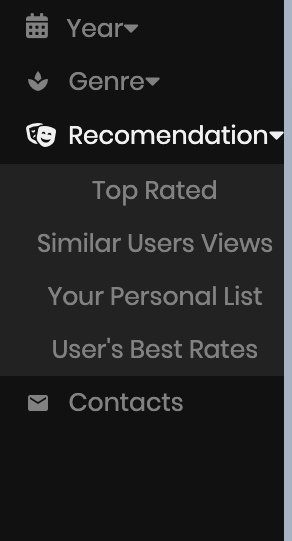
\includegraphics[scale=0.25]{9.png}
\end{figure}

Outra alternativa para procurar filmes é através da \textit{search bar}, onde o utilizador introduz uma palavra, e todos os filmes com essa palavra associada são apresentados.


\begin{figure}[H]
\centering
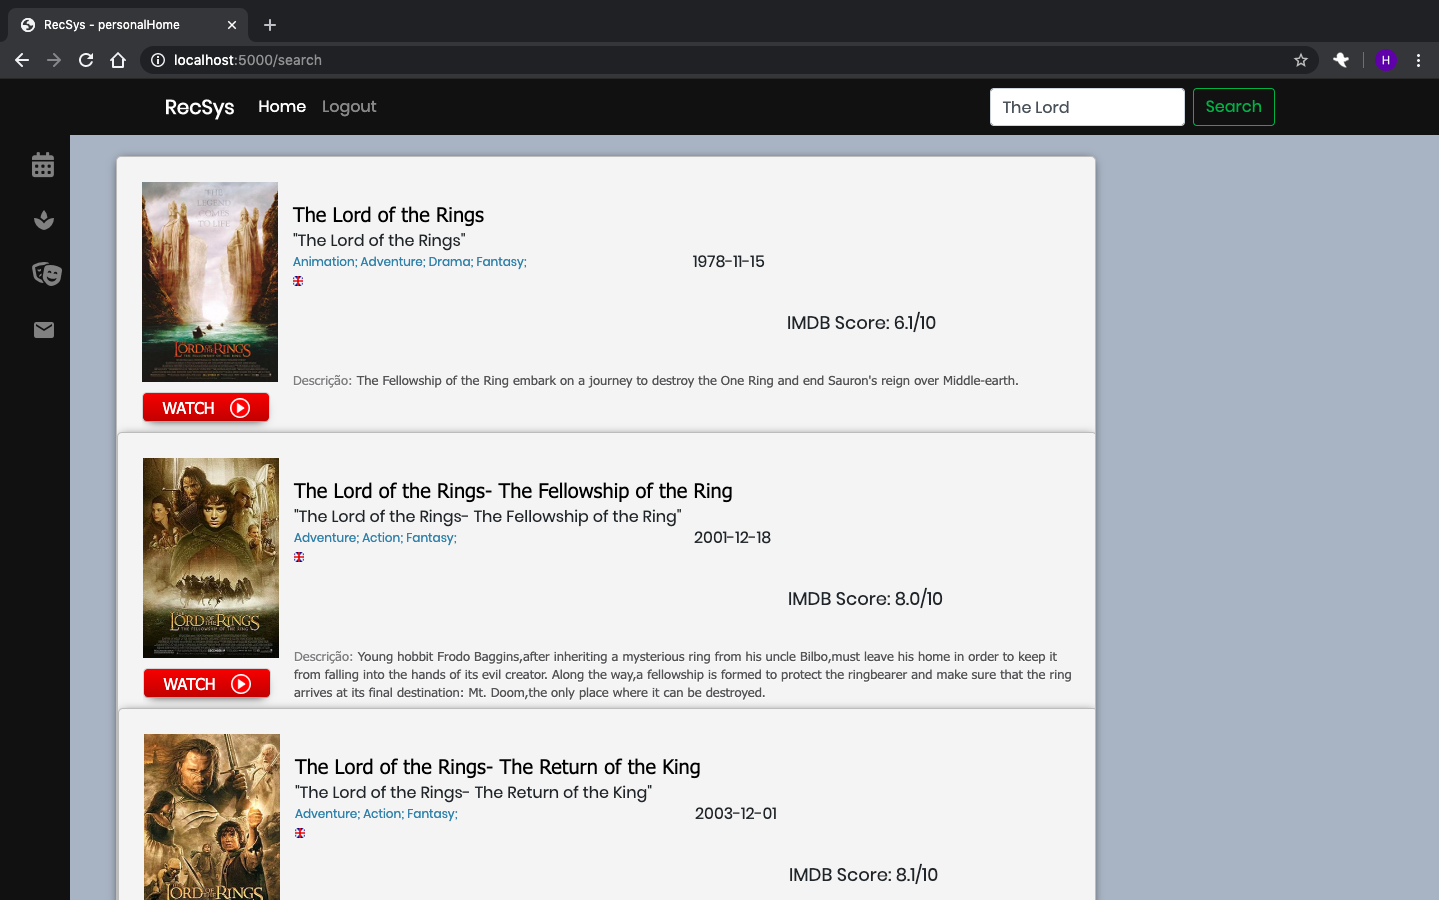
\includegraphics[scale=0.3]{5.png}
\end{figure}

O utilizador poderá também atribuir uma pontuação (1 a 5 estrelas).

\begin{figure}[H]
\centering
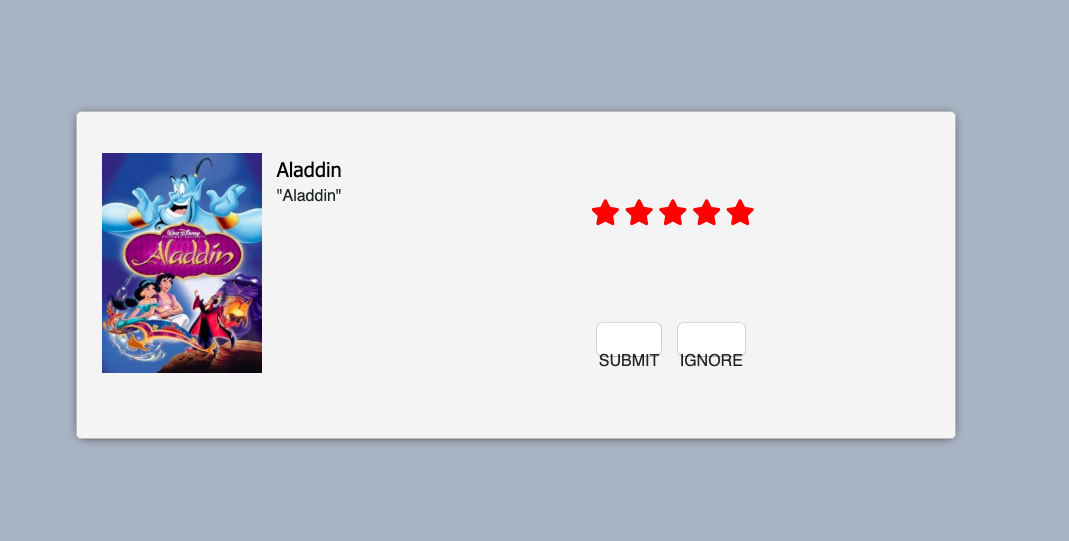
\includegraphics[scale=0.3]{6.png}
\end{figure}

Sempre que um utilizador atribui uma pontuação a um filme é adicionada informação à base de dados. Por exemplo, se um utilizador x que viu um filme y e atribuiu uma pontuação z, esta a informação fica guardada.

